\documentclass[11pt,a4paper]{article}
\usepackage[utf8]{inputenc}
\usepackage[T1]{fontenc}
\usepackage{array}
\usepackage{amsmath}
\usepackage{amsfonts}
\usepackage{siunitx}
\usepackage{placeins}
\usepackage{amssymb}
\usepackage{makeidx}
\usepackage{sidecap}
\usepackage{fvextra}
\usepackage{multicol}
\usepackage{listings}
\usepackage{appendix}
\usepackage{comment}
\usepackage{nicematrix}
\usepackage{multirow}
\usepackage{braket}
\usepackage{graphicx}
\usepackage{relsize}
\usepackage{fancyhdr}
\usepackage{cprotect}
\usepackage{color} 
\usepackage{hyperref}
\hypersetup{
	colorlinks=true, 
	linktoc=all, 
	linkcolor=blue,
	urlcolor=blue
}
\usepackage[left=2cm,right=2cm,top=1.5cm,bottom=2cm]{geometry}
\usepackage{titling}
\usepackage{etoolbox}
\flushbottom
\title{Statistical Analysis of Experimental Data\\
	\vspace{0.2cm}
	\large{Homework 05}}
\vspace{-0.2cm}
\author{Igor Di Tota}
\date{\small \url{https://github.com/igordt/SAED_homeworks/tree/main}}


\begin{document}
	\maketitle
	
	\section*{Introduction}

	This homework concerns Monte Carlo integration: \textit{use Monte Carlo method to calculate volume of a solid constructed as an intersection of three cones inside the unit cube, with unit diameters and unit heights, and perpendicular axes.}

	The cube occupies the region $[0,1]^3$, so that $V_{\text{cube}} = 1$.
	The solid considered is the set of points belonging to all three cones at the same time.
	Its volume is estimated by generating random points uniformly inside the cube and counting the fraction that falls inside the solid.
	\section*{Geometry of the problem}

	For a cone with axis along the coordinate $x_k$ ($k = 0, 1, 2$ for $x, y, z$), the base of radius $R = 1/2$ lies on a face of the cube and the apex at the centre of the opposite face, at distance $H = 1$ from the base.
	It is chosen that for the cones along $x$ and $z$ the base lies on the face $x_k = 0$ and the apex on the face $x_k = 1$, while for the cone along $y$ the base lies on the face $y = 1$ and the apex on the face $y = 0$.

	Let $t$ be the coordinate along the axis, measured from the base, and $(u, v)$ the two remaining coordinates.
	At height $t$, the cross-section of the cone is a disc centred on the axis, $(u, v) = (1/2, 1/2)$, whose radius decreases linearly from $R$ at the base to $0$ at the apex:
	\begin{equation}
		r(t) = R \left(1 - \frac{t}{H}\right).
	\end{equation}
	A point is therefore inside the cone if its distance from the axis does not exceed $r(t)$:
	\begin{equation}
		\left(u - \tfrac{1}{2}\right)^2 + \left(v - \tfrac{1}{2}\right)^2 \le R^2 \left(1 - \frac{t}{H}\right)^2 .
	\end{equation}
	Explicitly, for the three cones:
	\begin{equation}
		\begin{aligned}
			\text{cone } x: &\quad (y - \tfrac12)^2 + (z - \tfrac12)^2 \le \tfrac14 (1 - x)^2, \\
			\text{cone } y: &\quad (z - \tfrac12)^2 + (x - \tfrac12)^2 \le \tfrac14\, y^2, \\
			\text{cone } z: &\quad (x - \tfrac12)^2 + (y - \tfrac12)^2 \le \tfrac14 (1 - z)^2 .
		\end{aligned}
	\end{equation}
	The solid is the set of points satisfying all three conditions at the same time.

	\subsection*{Implementation}

	The functions used in the code are written for a cone with a generic axis $x_k$, so that the same code is reused for all three cones by changing the index $k$.
	The two coordinates perpendicular to the axis are obtained cyclically as $x_{(k+1) \bmod 3}$ and $x_{(k+2) \bmod 3}$.

	The function \texttt{inside} takes an array of points of shape $(3, N)$ and applies the condition derived above, returning a boolean mask that is \texttt{True} for the points inside the cone.
	The intersection of the three cones is then simply the logical AND of the three masks.
	The option \texttt{flip} moves the base to the opposite face, replacing $t \to 1 - t$; it is used for the cone along $y$.

	To draw the cones, the lateral surface is described in parametric form, with the coordinate along the axis $t$ and the azimuthal angle $\varphi$ around the axis:
	\begin{equation}
		t \in [0, H], \quad \varphi \in [0, 2\pi]: \qquad
		x_k = t, \quad
		u = \tfrac12 + r(t)\cos\varphi, \quad
		v = \tfrac12 + r(t)\sin\varphi .
	\end{equation}
	On a grid of values of $(t, \varphi)$, the three coordinates are computed and placed in the correct order according to the direction of the axis.
	The three cones, separately and together inside the cube, are shown in Figures~\ref{fig:single_cones} and \ref{fig:cones}.

	\begin{figure}[!h]
		\centering
		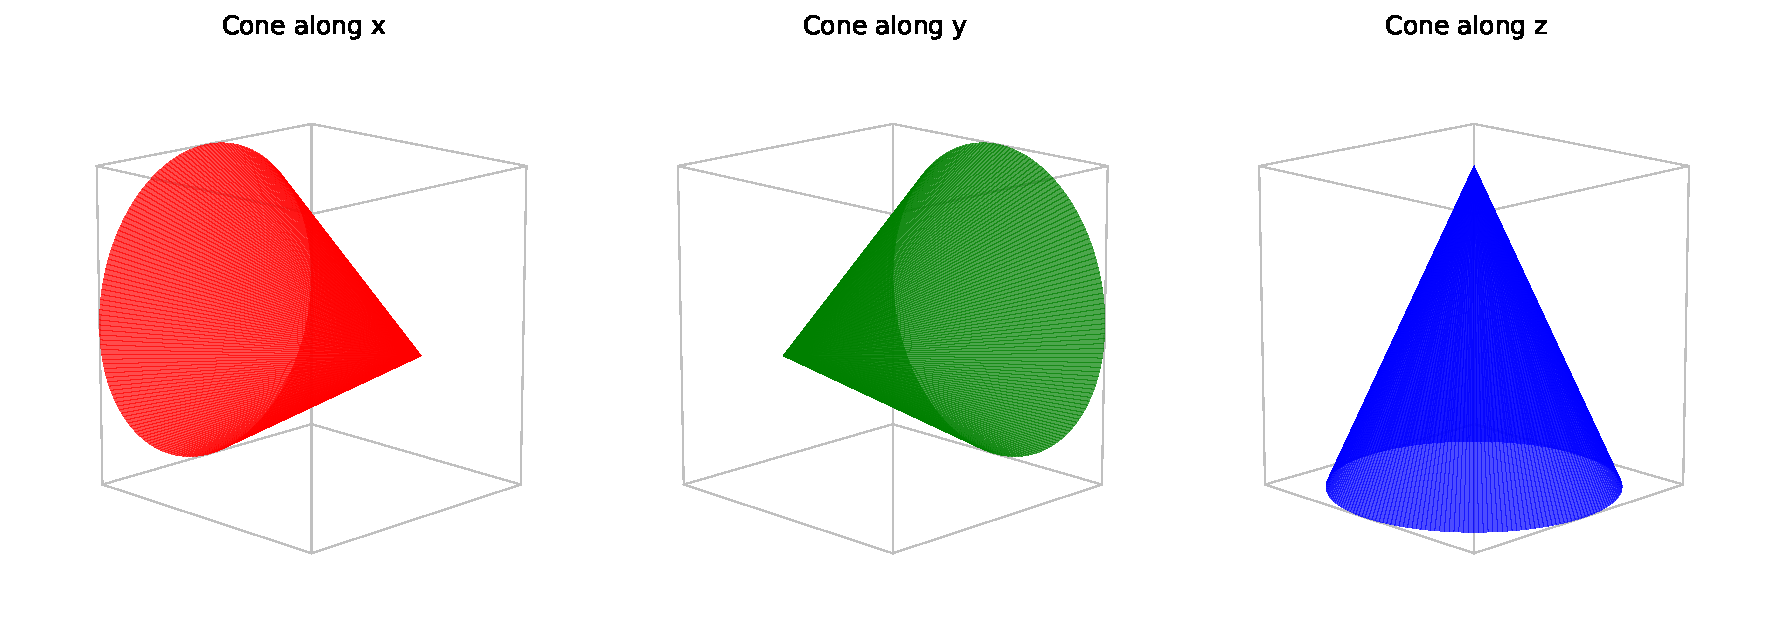
\includegraphics[width=\linewidth]{images/single_cones.pdf}
		\caption{The three cones inside the unit cube, with axes along $x$ (red), $y$ (green) and $z$ (blue).}
		\label{fig:single_cones}
	\end{figure}

	\begin{figure}[!h]
		\centering
		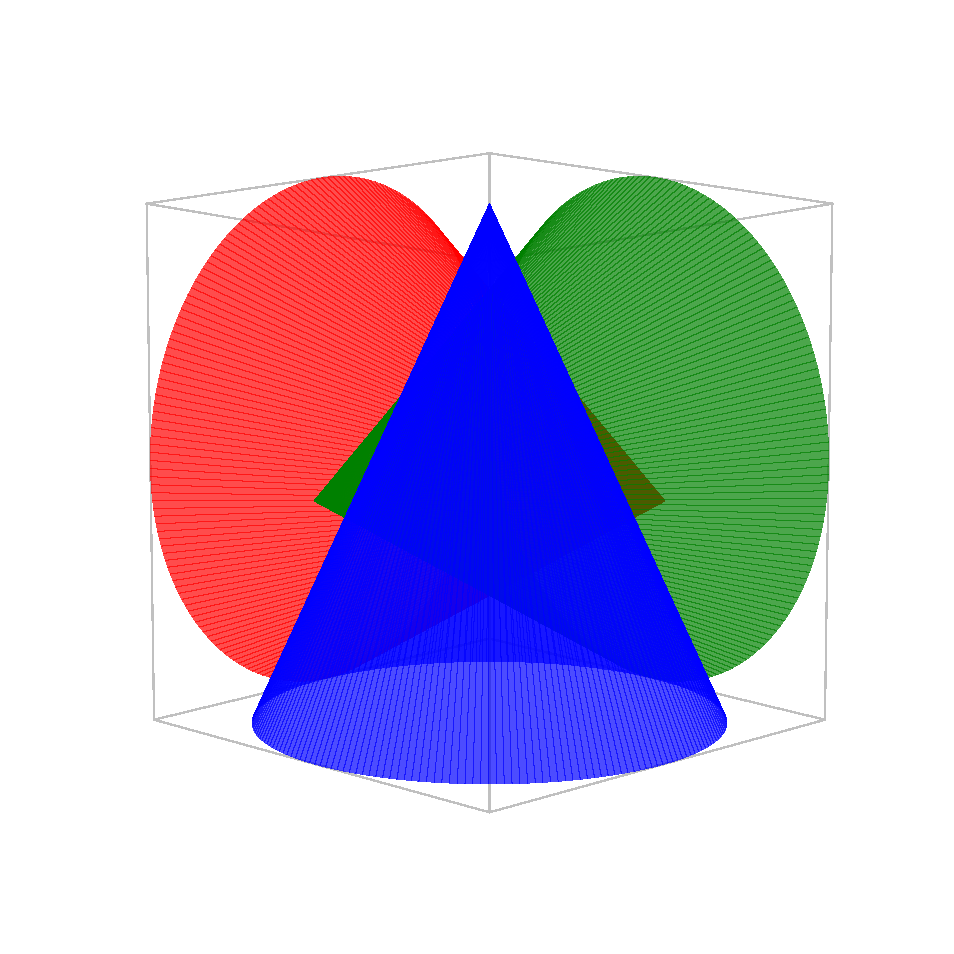
\includegraphics[width=0.5\linewidth]{images/cones.pdf}
		\caption{The three cones drawn together inside the unit cube. The solid is the region common to all three.}
		\label{fig:cones}
	\end{figure}
	\FloatBarrier

	\section*{Monte Carlo integration}

	The volume is estimated with the \textit{hit-or-miss} method seen in the lecture.
	$N$ points are generated uniformly inside the unit cube, drawing each coordinate independently from the uniform distribution on $[0, 1)$.
	For each point it is checked whether it lies inside the solid, and the number of accepted points $N_f$ is counted.

	Since the points are uniformly distributed, the probability for a point to be accepted is the ratio between the volume of the solid and the volume $I_0$ of the region where the points are generated:
	\begin{equation}
		p = \lim_{N \to \infty} \frac{N_f}{N} = \frac{V}{I_0}.
	\end{equation}
	Here the points are generated in the whole cube, so $I_0 = V_{\text{cube}} = 1$.
	The volume is then estimated as
	\begin{equation}
		V = \frac{N_f}{N} \, I_0 = \hat{p} \, I_0 .
	\end{equation}
	Each point is accepted or rejected independently with the same probability $p$, so $N_f$ follows a binomial distribution with variance $N p (1 - p)$.
	For $N \gg 1$, the uncertainty on the volume is therefore
	\begin{equation}
		\sigma_V = \sqrt{\frac{\hat{p}(1 - \hat{p})}{N}} \; I_0 .
		\label{eq:sigma}
	\end{equation}
	The uncertainty decreases as $1/\sqrt{N}$, independently of the number of dimensions of the problem.

	\subsection*{Validation on a single cone}

	Before computing the volume of the solid, the method is checked on a single cone, whose volume is known exactly:
	\begin{equation}
		V_{\text{cone}} = \frac{1}{3} \pi R^2 H = \frac{\pi}{12} \approx 0.26180 .
	\end{equation}
	The check is done on the cone with axis along $z$: the difference from the exact value is compared with the statistical uncertainty through the normalised residual
	\begin{equation}
		r = \frac{V_{\text{MC}} - V_{\text{exact}}}{\sigma_V} ,
	\end{equation}
	which should be of order 1 if the method and its uncertainty are correct.
	
	With $N = 10^6$ points the result is
	\begin{equation}
		V_{\text{MC}} = 0.26243 \pm 0.00044, \qquad V_{\text{MC}} - V_{\text{exact}} = 0.00063, \qquad r = 1.44 ,
	\end{equation}
	so the estimate agrees with the exact value within $\sim 1.4\,\sigma$.

	The generated points are shown in Figure~\ref{fig:cone_points}: the accepted points fill the volume of the cone, while the rejected ones fill the rest of the cube.

	\begin{figure}[!h]
		\centering
		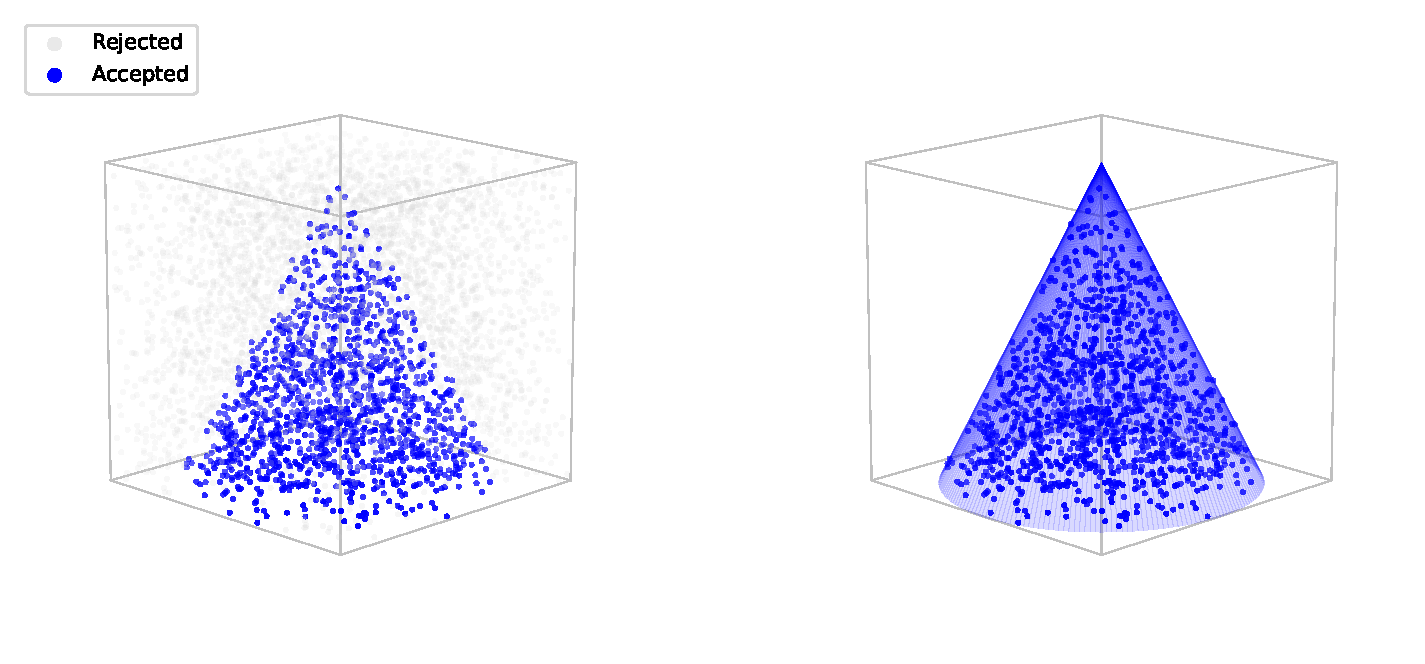
\includegraphics[width=0.85\linewidth]{images/cone_points.pdf}
		\caption{Left: the first $5000$ generated points, accepted (blue) and rejected (grey) for the cone along $z$. Right: only the accepted points.}
		\label{fig:cone_points}
	\end{figure}
	\FloatBarrier

	\section*{Volume of the intersection}

	The volume of the solid is estimated with the same procedure.
	A point is accepted only if it lies inside all three cones, i.e.\ the acceptance mask is the logical AND of the three masks:
	\begin{equation}
		\text{accepted} = \text{cone}_x \wedge \text{cone}_y \wedge \text{cone}_z .
	\end{equation}
	Using $N = 10^7$ points, $N_f = 609\,262$ are accepted, which gives $\hat{p} = 0.06093$ and
	\begin{equation}
		V = 0.06093 \pm 0.00008 ,
	\end{equation}
	with a relative uncertainty of $0.12\%$.
	The accepted points are shown in Figure~\ref{fig:solid_points}.

	\begin{figure}[!h]
		\centering
		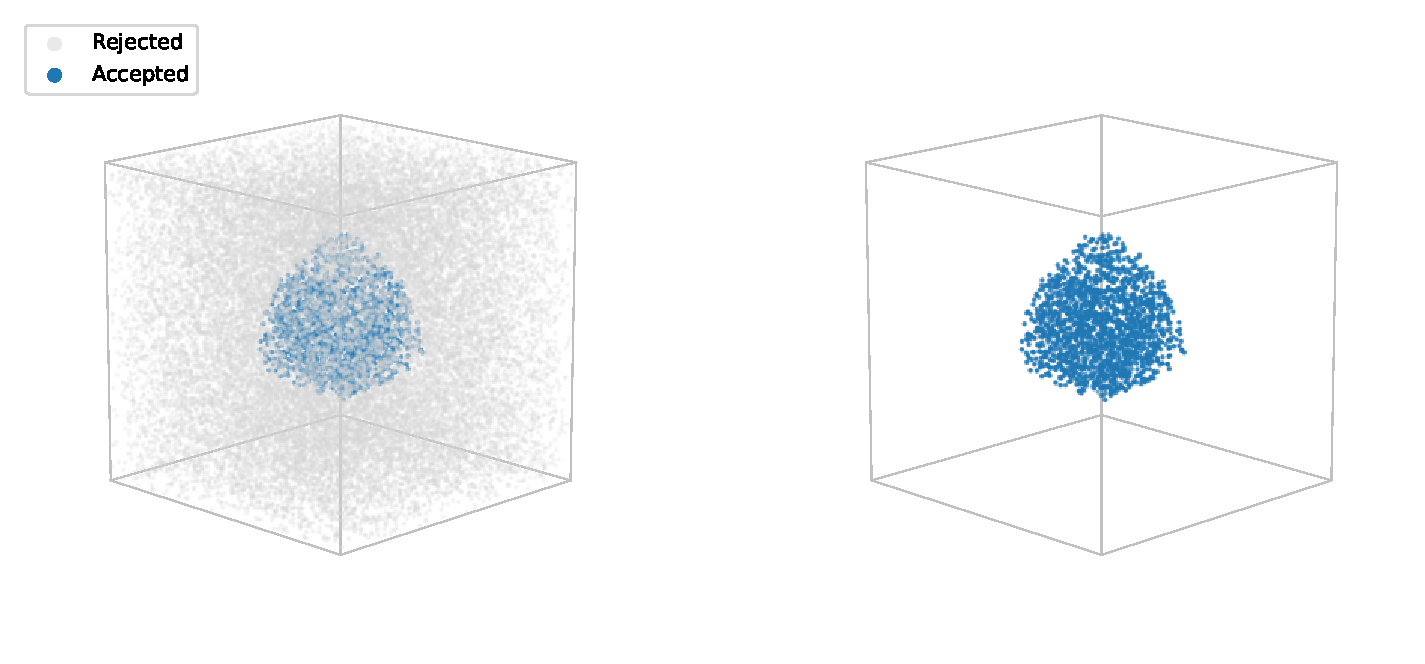
\includegraphics[width=0.85\linewidth]{images/solid_points.pdf}
		\caption{Left: the first $30000$ generated points, accepted (blue) and rejected (grey) for the intersection of the three cones. Right: only the accepted points, which show the shape of the solid.}
		\label{fig:solid_points}
	\end{figure}
	\FloatBarrier

	\section*{Convergence study}

	To study how the estimate depends on the number of generated points, the volume and its uncertainty are computed using only the first $N$ points of the sample, for values of $N$ from $10^2$ to $10^7$, equally spaced on a logarithmic scale.
	For each $N$, the binomial uncertainty of Eq.~\eqref{eq:sigma} gives
	\begin{equation}
		\frac{\sigma_V}{V} = \sqrt{\frac{1 - \hat{p}}{N \hat{p}}} \propto \frac{1}{\sqrt{N}} ,
	\end{equation}
	so on a logarithmic scale the relative uncertainty is expected to follow a straight line with slope $-1/2$.
	The expected curve is obtained by using the best estimate of $p$, from the full sample of $10^7$ points.
	The exact volume is not known, so the estimates are compared with this same best estimate.
	The results are shown in Figure~\ref{fig:convergence}, and some of them are reported in Table~\ref{tab:convergence}.

	\begin{figure}[!h]
		\centering
		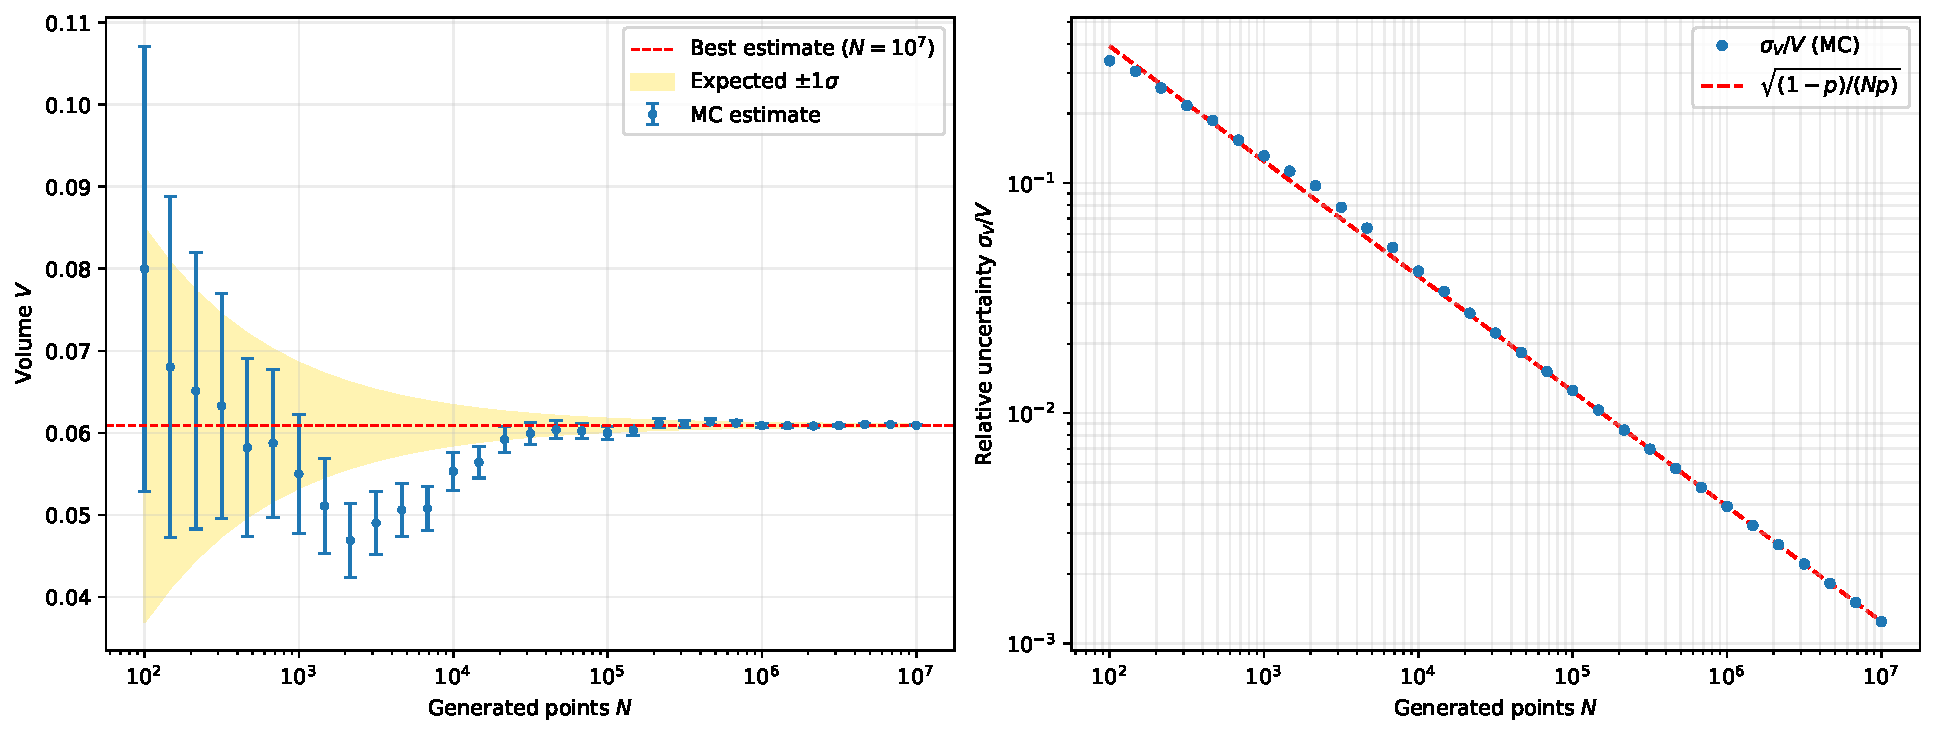
\includegraphics[width=\linewidth]{images/convergence.pdf}
		\caption{Left: volume estimate as a function of the number of generated points $N$, compared with the best estimate (dashed line) and with its expected $\pm 1\sigma$ band. Right: relative uncertainty as a function of $N$, compared with the expected $1/\sqrt{N}$ behaviour.}
		\label{fig:convergence}
	\end{figure}

	\begin{table}[!h]
		\centering
		\begin{tabular}{r r c c c}
			\hline
			$N$ & $N_f$ & $V$ & $\sigma_V$ & $\sigma_V / V$ \\
			\hline
			$100$        & $8$        & $0.08000$ & $0.02713$ & $33.91\,\%$ \\
			$681$        & $40$       & $0.05874$ & $0.00901$ & $15.34\,\%$ \\
			$4642$       & $235$      & $0.05062$ & $0.00322$ & $6.36\,\%$ \\
			$31623$      & $1895$     & $0.05992$ & $0.00133$ & $2.23\,\%$ \\
			$215443$     & $13193$    & $0.06124$ & $0.00052$ & $0.84\,\%$ \\
			$1467799$    & $89332$    & $0.06086$ & $0.00020$ & $0.32\,\%$ \\
			$10000000$   & $609262$   & $0.06093$ & $0.00008$ & $0.12\,\%$ \\
			\hline
		\end{tabular}
		\caption{Volume estimate and its uncertainty for some values of the number of generated points $N$.}
		\label{tab:convergence}
	\end{table}
	\FloatBarrier

	\section*{Conclusions}

	The volume of the solid obtained as the intersection of three perpendicular cones inside the unit cube was estimated with the hit-or-miss Monte Carlo method.

	The method was first validated on a single cone: with $N = 10^6$ points the estimate $V = 0.26243 \pm 0.00044$ agrees with the exact value $\pi/12 \approx 0.26180$ within $1.4\,\sigma$.

	Using $N = 10^7$ points, of which $N_f \approx 6.09 \times 10^5$ were accepted, the volume of the solid is
	\begin{equation}
		V = 0.06093 \pm 0.00008 ,
	\end{equation}
	with a relative uncertainty of about $0.12\%$.

	The convergence study shows that the relative uncertainty decreases as $1/\sqrt{N}$, as expected from the binomial distribution of the number of accepted points.
	The estimates obtained with fewer points fluctuate around the final value, compatibly with their uncertainties.

\end{document}
